\documentclass[Bachelorarbeit.tex]{subfiles}
\begin{document}
\chapter{Implementierung}
\label{chap:implementierung}

Ziel dieses Kapitel ist es, einen Überblick über die Implementierung der verschiedenen Plattformen zu geben.
Hierzu wurde das Kapitel in zwei Abschnitte unterteilt, die stellvertretend für die zwei Subsysteme \nameref{sec:android_app} und \nameref{sec:wp_app} stehen, aus welchen sich das Projekt zusammensetzt.
Anhand des definierten Szenarios Login (siehe Abschnitt: \ref{sec:usecases} - \nameref{sec:usecases} des \ref{chap:entwicklung}. Kapitels) soll die \nameref{chap:implementierung} durch die einzelnen Schichten der Applikationen aufgezeigt werden.
Des weiteren werden in den Abschnitten \ref{sec:android_app} - \nameref{sec:android_app} und \ref{sec:wp_app} - \nameref{sec:wp_app} die plattformspezifischen Besonderheiten der grafischen Oberfläche behandelt.


\section{Android Applikation}
\label{sec:android_app}

\subsection*{Grafische Oberfläche}
Android bietet über das \ac{SDK} ein reichhaltiges Angebot für die Gestaltung des \ac{UI} an.
Durch die kontinuierlichen Erweiterungen der \ac{UI}-Bibliotheken werden regelmäßig neue Konzepte (siehe Abschnitt \nameref{subsubsec:fragments}) sowie Features vorgestellt.
Diese sind neben weiteren Änderungen Bestandteil der jeweiligen \ac{API}-Version des \ac{SDK}.
Das Mindest- sowie das Ziel-\ac{API}-Level werden im Manifest\footnote{Das Manifest ist eine \ac{XML}-Datei in welcher die Rahmenbedingungen der App definiert werden.} des Projektes festgelegt. 
Dabei gibt das Ziel-\ac{API}-Level an, für welche Android Version die Applikation optimiert ist. 
Dagegen definiert das Mindest-\ac{API}-Level die älteste Android Version, unter welcher die Applikation vollständig lauffähig ist.
Je nach gewählter Spezifikation wird die Auswahl der möglichen Optionen durch das \ac{API}-Level eingeschränkt. 
Deshalb gilt es abzuwägen, ob eher die \texttt{breite Masse} (niedriges \ac{API}-Level) erreicht werden soll, oder ob der Fokus auf der Verwendung von modernen Gestaltungselemente (hoher \ac{API}-Level) liegt.
Des weiteren wird für die \ac{UI}-Entwicklung eine Support-Bibliothek durch das Android-\ac{SDK} zur Verfügung gestellt. 
Mithilfe derer ist es möglich, eine Abwärtskompatibilität bis zu  \ac{API}-Level 4 (Android 1.6) sicherzustellen. \parencite[vgl.:][]{android_supportLib}\\

\subsubsection*{Activities}
\label{subsubsec:activities}
Eine Activity ist eine in sich geschlossene Komponente, welche eine grafische Oberfläche an die Applikation anbindet.
Eine Activity besteht aus einer Java- sowie \ac{XML}-Datei.
Zum einen erfolgt in der Java-Datei die Anbindung der Activity an die Applikation. 
Zum anderen kann auf die einzelnen \ac{UI}-Elemente zugegriffen und deren  Verhalten definiert werden.
Die \ac{XML}-Datei dient der Gestaltung der grafischen Benutzeroberfläche.
Neben der Spezifikation der anzuzeigenden \ac{UI}-Elementen können an dieser Stelle auch Designeinstellungen vorgenommen werden.
Die \ac{XML}-Datei kann entweder mit einem Text-Editor oder mithilfe eines \ac{UI}-Designers der jeweiligen \ac{IDE} erzeugt und bearbeitet werden.\\
\\
In der Beispiel-Applikation wurde für jedes Szenario (siehe Abschnitt: \nameref{sec:usecases} des \ref{chap:entwicklung}. Kapitels) eine eigene Activity erstellt.\footnote{Details zur Verwendung von \nameref{subsubsec:activities} in der Beispiel-Applikation befinden sich in dem Abschnitt: \nameref{subsec:login_android} des \ref{chap:implementierung}. Kapitels}. 
Damit ergibt sich ein modularer Aufbau, wodurch der Funktionsumfang der Applikation einfach erweitert werden kann.

\subsubsection*{Fragments}
\label{subsubsec:fragments}
Das Konzept der \nameref{subsubsec:fragments} wurde offiziell mit dem Erscheinen von Android3 in das \ac{SDK} aufgenommen. Durch den Einsatz der \texttt{Support Library} ist es möglich, \nameref{subsubsec:fragments} auch in älteren Android-Versionen einzusetzen.
Mithilfe von \nameref{subsubsec:fragments} lässt sich der Inhalt beziehungsweise das Verhalten in einzelne Komponenten aufteilen.
Dadurch besteht die Möglichkeit, eigenständige und wiederverwertbare Inhalte zu erzeugen. 
Da \nameref{subsubsec:fragments} die Teilmenge einer Activity bilden, sind sie neben ihrem eigenen \texttt{Lifecycle} auch von dem \texttt{Lifecycle} der jeweiligen Activity abhängig.\\
\newpage
Für die Kommunikation zwischen verschiedenen Fragments ist es zu  empfehlen, einen \texttt{Callback}-Mechanismus in die übergeordnete Activity zu implementieren.
\parencites()()[vgl.:][Seite 96: Fundamental Android UI Designs]{android_profDev}[sowie:][]{android_fragments} \\
\\
In der Beispiel-Anwendung wurden in jeder Activity  \nameref{subsubsec:fragments} eingesetzt. 
Der Sinn von Fragments wird an folgenden Beispiel klarer ersichtlich. \\
\\
Nach dem erfolgreichen Login (Activity) wird in der Beispiel-Applikation der Startbildschirm (Activity) aufgebaut, dieser wird durch zwei \nameref{subsubsec:fragments} dargestellt. 
Hierbei werden in dem ersten Fragment die offenen- und im zweiten Fragment die bearbeiteten Veranstaltungen angezeigt (siehe Abb.: \ref{fig:mockup_android_dashboard} - \nameref{fig:mockup_android_dashboard} im Anhang: \nameref{chap:diagramme_und_bilder}).
Zwischen den beiden \nameref{subsubsec:fragments} kann mit einer Wischbewegung gewechselt oder eine zu bearbeitende Veranstaltung ausgewählt werden.

\begin{comment}
\paragraph*{Aufruf der Activity}

\begin{itemize} \color{red}
\item Erläuterung der Callback-Methoden
\end{itemize}
\end{comment}

\subsection*{Login Szenario - Android Applikation}
\label{subsec:login_android}

In diesem Abschnitt soll die Implementierung des Login-Szenarios (siehe Abschnitt: \nameref{sec:usecases} des \ref{chap:entwicklung}. Kapitels)  für die Android-Applikation demonstriert werden. 
Zum einen werden dabei die verwendeten Android-Werkzeuge und zum anderen die implementierte Architektur beschrieben. 


\begin{comment}
\begin{itemize} \color{red}
\item Übersicht der Verwendeten Techniken und Beschreibung
\begin{itemize}
\item \nameref{subsub:android_service}
\item \nameref{subsub:android_uc-controller}
\item \nameref{subsub:android_async-task}
\end{itemize}
\end{itemize}
\end{comment}

\subsubsection*{Service}
\label{subsub:android_service}

Grundsätzlich gibt es zwei Arten von Services in Android: \texttt{Local}- und \texttt{Remote}-\nameref{subsub:android_service}s.
Der \texttt{Local}-\nameref{subsub:android_service} kann wiederum in die zwei Unterkategorien \texttt{Started}  und \texttt{Bound} eingeteilt werden.
Ein \texttt{Started}-\nameref{subsub:android_service} wird explizit von der Anwendung gestartet und beendet\footnote{Das Verhalten des Start- und Endzeitpunkt lassen sich durch Parameter anpassen.}, während ein \texttt{Bound}-\nameref{subsub:android_service} nur ausgeführt wird solang eine Komponente an ihn gebunden ist (siehe Abb.: \ref{fig:service_lifecycle} - \nameref{fig:service_lifecycle} im Anhang: \nameref{chap:diagramme_und_bilder}).  
Der Vorteil eines \texttt{Remote}-\nameref{subsub:android_service} liegt darin, dass fremde Android-Applikation auch auf diesen zugreifen können.
\parencites()()[vgl.:][]{android_service}[sowie:][ab Seite: 409ff]{android_proAndroid4}\\
\\
Innerhalb der Beispiel-Applikation wird ein \texttt{Bound}-\nameref{subsub:android_service} für Datebank- und Webservice-Zugriffe eingesetzt. 
Nach dem Starten der Login-Activity bindet sich die Activity mithilfe des bereitgestellten Interfaces auf den\\ \texttt{EventDokuService}.
Sobald der Sende-Button gedrückt wurde, ruft die Login-Activity die Methode \texttt{login} des Services auf und übergibt diesem die entsprechenden Daten.  
Der Service gibt darauf hin die Daten an den Login-\nameref{subsub:android_uc-controller} weiter.
Dieser bearbeitet die Anfrage und leitet, nach der Fertigstellung, das Ergebnis direkt an die Login-Activity weiter.

\subsubsection*{Usecase-Controller}
\label{subsub:android_uc-controller}
Ein \nameref{subsub:android_uc-controller} implementiert die Logik und den Ablauf eines definierten Szenarios (siehe Abschnitt: \nameref{sec:usecases} des \ref{chap:entwicklung}. Kapitels). 
Der Ablauf des \nameref{subsub:android_uc-controller} wird über eine Fassade von dem Service gestartet.
Dabei wird in der Fassade jeder Controller nach dem \texttt{Singleton}-Muster gehalten. 
Zu Beginn des Ablaufes eines \nameref{subsub:android_uc-controller}s wird ein Container-Objekt mit den erhaltenen Daten erzeugt. 
Dieser Container wird, solange kein Fehler auftritt, durch die Liste der abzuarbeitenden Aufgaben  gereicht.
Bei jedem Schritt (Aufgabe) werden entsprechenden Informationen dem Container hinzugefügt oder abgeändert.
Das Schema des \nameref{subsub:android_uc-controller} ist Bestandteil der entwickelten Architektur und nicht des Android-\ac{SDK}'s.\\
\\
Im Falle des Login-Szenarios verfügt der Controller über zwei Aufgaben, welche asynchron ausgeführt werden.
Im ersten Schritt \texttt{getRandomNumber} wird eine Zufallszahl über den Webservice von dem Server angefordert. 
Diese Zahl ist für das \texttt{hashen} des Passworts notwendig, welches wiederum im nächsten Schritt benötigt wird.
Nach Erfolg des ersten Schrittes wird der zweite eingeleitet.
Dabei wird wiederholt auf den Webservice zugegriffen. 
Zusätzlich werden diesmal die benötigten Zugangsdaten mitgesendet um sich am Server zu authentifizieren.
Sollte die Authentifikation erfolgreich verlaufen sein, so wird der  retourniert Token in dem Laufzeitspeicher der Applikation abgelegt.
Die Login-Activity wird anschließend durch ein \texttt{Callback-Interface} über den positiven- oder negativen Verlauf des Szenarios informiert und kann dementsprechend fortfahren. 

\subsubsection*{Asynchrone Tasks}
\label{subsub:android_async-task}

Da ein \nameref{subsub:android_service} standardmäßig im \texttt{Haupt-Thread} läuft, wird während der Arbeiten im Backend das \ac{UI} der Applikation blockiert.
Dies macht sich vor allem bei Zugriffen auf externe Informationen, wie beispielsweise dem Webservice oder die Datenbank, bemerkbar.
Neben der schlechten Usability liegt ein weiteres Problem darin, dass bei zu lange gesperrten Applikationen das Betriebssystem einen \ac{ANR}-Dialog erzeugt. \parencite[vgl.][]{android_responsive}
Um dieser Problematik vorzubeugen bietet das \ac{SDK} verschiedenen Lösungen an.
Innerhalb der Beispiel-Applikation wurden  \texttt{AsyncTask}'s für die einzelnen Aufgaben der Controller (siehe Abschnitt: \nameref{subsub:android_uc-controller} eingesetzt.
Dadurch ist es möglich, zeitintensive Aufgaben in Hintergrund-Operationen auszulagern, ohne dabei die Applikation zu blockieren.


\section{Windows Phone Applikation}
\label{sec:wp_app}

In diesem Abschnitt wird die Implementierung der Beispiel-Applikation EventDoku als \ac{WP}8 App betrachtet. 
Bei der Entwicklung für die \ac{WP}-Plattform ist der Einsatz von Visual Studio als \ac{IDE} zu empfehlen. 
An dieser Stelle sollte erwähnt werden, dass das Einrichten der Entwicklungsumgebung nicht ganz problemlos von der Hand geht.
Die Problematik liegt in dem Ausführen sowie Testen der Applikation.
Grundsätzlich kann die Entwicklung im Emulator oder auf einem \ac{WP}8-Gerät ausgeführt werden. 
Allerdings gibt es bei beiden Möglichkeiten gewisse Hürden, welche in dem Abschnitt: \nameref{sub:wp_entwicklung} des \ref{chap:state_of_the_art}. Kapitels (\nameref{chap:state_of_the_art}) genauer betrachtet werden.
  


\subsection*{Grafische Oberfläche}


EntwicklerInnen, die über Erfahrung mit dem \ac{WPF}-Framework verfügen, werden sich in der \ac{WP}-Entwicklung schnell zurecht finden.
Durch die Nähe zum \texttt{.NET}-Framework kann für die Implementierung einer \ac{MVVM}-Architektur auch auf bekannte Konzepte, wie zum Beispiel \texttt{Databinding}, zurück gegriffen werden. 
Wie auch in der Android-Entwicklung stehen für die Erzeugung eines neuen \ac{WP}-Projektes bestehende Templates bereit, die als Grundgerüst einer Applikationen verwendet werden können.
 
\subsubsection*{Application Page}
\label{subsubsec:application-page}

Die \texttt{PhoneApplicationPage} stellt einen wiederverwendbaren \ac{UI}-Container dar. 
Eine \ac{WP}-Application Page kann als Äquivalent zu den Android-\nameref{subsubsec:activities} betrachtet werden \parencite[vgl.:][]{wp8_vglAndroid}. 
Ähnlich wie bei einer Android-Anwendung besteht die grafische Oberfläche einer \ac{WP}8-Applikation aus einer Design- sowie einer Code-basierten Datei. 
Um das Design zu definieren kann die \ac{XAML}-Beschreibungssprache verwendet werden. 
Für diesen Zweck ist es möglich, den integrierten Visual Studio-Designer oder Microsoft Blend einzusetzen.
Für die Anbindung des \ac{UI} an die Applikation wird die in  \texttt{C\#} geschriebene \texttt{Codebehind}-Datei verwendet.\\
\\
In der Beispiel-Applikation wurde für jedes Szenario (siehe Abschnitt: \nameref{sec:usecases} des \ref{chap:entwicklung}. Kapitels) eine eigene \nameref{subsubsec:application-page} erstellt.
Parallel dazu wurde für jede \nameref{subsubsec:application-page}
ein eigenes \texttt{ViewModel} angelegt, das sich die Daten für Darstellung hält und aufbereitet.

\subsubsection*{Panorama Items}
\label{subsubsec:panorama-items}
Durch die \nameref{subsubsec:panorama-items} wird der Inhalt einer \nameref{subsubsec:application-page} in vertikal angeordnete Seiten aufgeteilt (siehe Abb.: \ref{fig:panorama-control} - \nameref{fig:panorama-control}). 
Dabei ist es möglich, die \nameref{subsubsec:panorama-items} so zu designen, dass sie als wiederverwertbare Module in den unterschiedlichen \nameref{subsubsec:application-page} eingesetzt werden können.  
\nameref{subsubsec:panorama-items} kann man vom Anwendungsprinzip  mit Android \nameref{subsubsec:fragments} vergleichen. \\
\\
In der Beispielanwendung wurden, bis auf den Login, alle \nameref{subsubsec:application-page} (Szenarios) in \nameref{subsubsec:panorama-items} unterteilt. 
Ein Beispiel dafür ist der nach dem erfolgreichen Login dargestellte Startbildschirm. 
Auf diesem werden in den ersten \nameref{subsubsec:panorama-items} die offenen und in den zweiten \nameref{subsubsec:panorama-items} die bearbeiteten Veranstaltungen dargestellt (siehe Abb.: \ref{fig:wp-startbildschirm} - \nameref{fig:wp-startbildschirm} im Anhang: \nameref{chap:diagramme_und_bilder}).
Für die Darstellung der Daten wurden Listenansichten gewählt, die jeweils an die oben erwähnten \texttt{ViewModels} gebunden sind.
Ziel dieses Vorgehen war es, das \ac{MVVM}-Muster in der \ac{WP}-Applikation zu implementieren.


\begin{figure}[h]
\centering
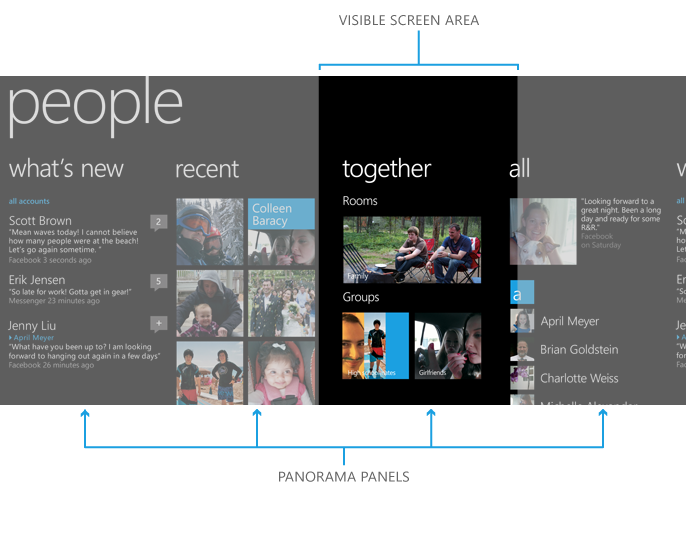
\includegraphics[width=0.7\linewidth]{./img/panorama-controll}
\caption[Panorama Controll]{Ansicht der Panorama Control mit ihren Panorama-Panels. \parencite[Quelle:][]{wp8_PanoramaControl}}
\label{fig:panorama-control}
\end{figure}


\begin{comment}
\subsubsection*{Navigation}

NavigationService ist in der Applikation schon integriert und muss nur mit dem Befehl \texttt{NavigationService.Navigate(URI von der \ac{XAML} der Page)}\\
Erste PanoramaItem wird standartmäßig geladen.\\
\\
BackButton ist default impl. springt auf die letzte Page zurück.
In der Applikation wurde der BackButton so implementiert das man von der Startseite (Dashboard) zurück auf den LoginPage kommt. \\
Von der LoginPage wird das Programm hart geschlossen (terminate).
\end{comment}

\subsection*{Login - Windows Phone Applikation}\label{subsec:login-wp}
An dieser Stelle wird die Implementierung des Login-Szenarios (siehe Abschnitt: \nameref{sec:usecases} des \ref{chap:entwicklung}. Kapitels)  für die \ac{WP}-Applikation demonstriert. 
Bei der Implementierung wurde versucht, einen Großteil der Backend-Logik aus der Android-Applikation für die \ac{WP}-App zu übernehmen, beziehungsweise diese zu portieren.
Durch dieses Vorgehen wurde ein einheitliches Backend erzeugt mit dem Ziel, die Wartbarkeit zu erhöhen und die Fehleranfälligkeit in der Logik zu minimieren. \\

\subsubsection*{Service}
Der hier verwendete Service ist nicht, wie im Android-Beispiel, ein Bestandteil des \ac{WP}-\ac{SDK}, sondern stellt eine implementierte Abstraktionsschicht der Backend-Architektur da.
Dabei besitzt die \texttt{Codebehind}-Datei eine Referenz auf den Service.
Mithilfe des \texttt{Singleton}-Musters wurde sichergestellt, dass maximal nur eine Initialisierung des Services existiert. \\
\\
Das Verhalten sowie die Implementierung des Service wurde größtenteils von der Android-Applikation (siehe Abschnitt: \nameref{subsec:login_android}) in die \ac{WP}-App übernommen.
Der Ablauf beziehungsweise die Logik des Login-Szenarios wurde in dem Punkt der Service-Portierung nicht verändert.\\
Das gleiche zählt auch für die \texttt{Usecase-Controller}, weshalb sie an dieser Stelle nicht wiederholt behandelt werden.
Weitere Information  bezüglich der \texttt{Usecase-Controller} befinden sich im Abschnitt: \nameref{subsec:login_android}.

\subsubsection*{Asynchrone Tasks}
Die Asynchrone Entwicklung wird für die gleichen Zwecke wie in der Android-Applikation benötigt. 
Allerdings  werden dafür die Bibliotheksfunktionen des \texttt{.NET}-Framework 4.5 (\texttt{async/await}) eingesetzt \parencite[vgl.:][]{wp8_async}.\\


\begin{comment}
Wenn Login ausgeführt wird, asyn aufruf des loadingScreen.
Wenn Succesful aufruf des Usecase LoadData.
WEnn negativ, Rücksprung auf Login mit benachrichtung.
\end{comment}


% Server wird rausgelassen 
\begin{comment}
\section{Server}
\label{sec:server}

\subsection*{Login}

\begin{itemize} \color{red}
\item Erläuterung der Serverseitigen Struktur anhand des Programmablaufs
\end{itemize}
\end{comment}

\end{document}